\documentclass[tikz,dvipsnames]{standalone}
\usetikzlibrary{backgrounds}
\usetikzlibrary{calc,positioning}

\begin{document}
 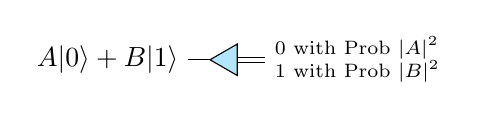
\begin{tikzpicture}[
    show background rectangle,
    tight background=0,
    background rectangle/.style={fill=white},
 ]
    \node[anchor=east] (X) {$A|0\rangle+B|1\rangle$};
    \coordinate (P) at ($(X)+(1.3,0)$);
    \coordinate (Q) at ($(P)+(0.2,0)$);
    \coordinate (Y0)at ($(X)+(2.0,+0.15)$);
    \coordinate (Y1)at ($(X)+(2.0,-0.15)$);
    
    \node[anchor=west] at (Y0) {\scriptsize 0 with Prob $|A|^2$};
    \node[anchor=west] at (Y1) {\scriptsize 1 with Prob $|B|^2$};
    \draw (X) -- (P);
    \draw (Q) ++(0,+0.03) -- ++(0.5,0);
    \draw (Q) ++(0,-0.03) -- ++(0.5,0);
    \filldraw[fill=cyan!30] (P) -- ++(30:0.4) -- ++(270:0.4) -- cycle;
    
\end{tikzpicture}
\end{document}
